\documentclass[twocolumn,prb,amsmath,amssymb,amsfonts,nobalancelastpage]{revtex4}
\usepackage{graphicx} 
\usepackage{xltabular}
\usepackage{booktabs}

\begin{document}

\title{Developing Early Warning Systems for Invasive Species Populations}

\author{Henry Traynor}
\affiliation{Odum School of Ecology, University of Georgia,
Athens, Georgia 30602\\}

\date{\textit{\today}}

\begin{abstract}

Lorem ipsum dolor sit amet, consectetur adipiscing elit, sed do eiusmod tempor incididunt ut labore et dolore magna aliqua. Gravida neque convallis a cras semper auctor neque vitae tempus. Auctor eu augue ut lectus arcu bibendum at varius vel. Et tortor at risus viverra adipiscing at in. Semper viverra nam libero justo laoreet sit amet cursus sit. Nunc mattis enim ut tellus elementum sagittis vitae. Sed enim ut sem viverra aliquet. Semper eget duis at tellus at urna condimentum mattis. Sagittis id consectetur purus ut faucibus pulvinar elementum integer enim. Molestie ac feugiat sed lectus vestibulum mattis ullamcorper velit sed.

\end{abstract}
%------------------------------------------------------------------
\maketitle
%-------------------------------------------------------
\section{Introduction}

The aim of this project is to develop early warning systems for invasive species population via analysis of a stochastic model. Models created using traditional Lotka-Volterra (LV) equations have been studied and analyzed extensively, though the literature remains sparse in the context of invasive species populations. The ability to predict large abundance spikes in invasive species has become increasingly necessary as climate change, increased artificial transfer of species, and habitat loss has allowed invasive species to wreak havoc on endemic individuals.

In our case, competition LV equations describe a two species system of competition over some common resource. The model is largely mechanism agnostic, meaning the intrinsic rate at which processes are happening is the only significant feature of the system to the output of the system of equations. It is important to note that this system is time-invariant (autonomous). 

%----------------------------------------------------------------
\section{Variable Definitions and Equation Set}
First, let us introduce the relevant variables for discussion and model creation.
\begin{xltabular}{\linewidth}{ l | X | X}
  \caption{Description of Variables used in this Study} 
 \label{table: vardescription}\\
 \hline \hline

\textbf{\normalsize Variable} & \textbf{\normalsize Definition} & \textbf{\normalsize Units} \\
 \hline 
\endfirsthead
 \hline \hline

\textbf{\normalsize Variable} & \textbf{\normalsize Definition} & \textbf{\normalsize Units} \\
 \hline 
\endhead

\textbf{$N_i$} & population size of species $i$ & Individuals\\ \hline 

\textbf{$\beta_i$} & per-capita growth rate of species $i$ & per time (year) \\ \hline 

\textbf{$K_i$} & carry capacity of species $i$ & individuals \\ \hline

\textbf{$\alpha_{ij}$} & interspecific competition factor of species $j$ on species $i$ & dimensionless \\ \hline

\end{xltabular}

Important notes on the table above: carrying capacity $K_i$ is the carry capacity of species $i$ given that there are no individuals from any other species present in the system; the dimensionless nature of $\alpha_{ij}$ arises from it simply being the negative scalar effect of the presence of an individual of species $j$ existing among a population of species $i$. This is analogous to opportunity cost in an economic framework.

Further comments of significance: from henceforth, species $i$ and species $j$ will be used in conjunction, as will species 1 and species 2. In both cases, species $i$ and species 1 are considered endemic populations and species $j$ and species 2 are considered invasive or "invaders."

The traditional LV model for competition is an expansion of the logistic population model:
$$\frac{dN_i}{dt}=\beta_i N_i(1-\frac{N_i}{K_i})$$

However, this neglects interspecific competition. To correct this and allow for a multi-species system, the equation above is revised to the following equations:
$$\frac{dN_i}{dt}=\beta_i N_i(1-\frac{N_i}{K_i}-\alpha_{ij}\frac{N_j}{K_i})$$
$$\frac{dN_j}{dt}=\beta_j N_j(1-\frac{N_j}{K_j}-\alpha_{ji}\frac{N_i}{K_j})$$

After distributing, these equations take the form
$$\frac{dN_i}{dt}=\beta_i N_i - \frac{\beta_i N_i^2}{K_i} - \alpha_{ij}\frac{\beta_i N_i N_j}{K_i}$$

Each term of the equation represents the species birth rate, death due to intraspecific competition rate, and death due to interspecific competition rate, respectively. It is important to delineate that the interspecific competition term represents the rate of death, whereas the interspecific competition factor is the scalar quantity $\alpha_{ij}$. This is the simplest form of the deterministic model.

\subsection{Deterministic Realizations}
Below is a graph of a realization of the deterministic model shown above using the following parameters:

\begin{xltabular}{\linewidth}{ X | X}
  \caption{Realization Parameters} 
 \label{table: vardescription}\\
 \hline \hline

\textbf{\normalsize Parameter} & \textbf{\normalsize Value} & \textbf{\normalsize Units} \\
 \hline 
\endfirsthead
 \hline \hline

\textbf{\normalsize Parameter} & \textbf{\normalsize Value} \\
 \hline 
\endhead

\textbf{initial $N_i$} & 700\\ \hline 

\textbf{initial $N_j$} & 5\\ \hline 

\textbf{$K_i$} & 700\\ \hline 

\textbf{$K_j$} & 700\\ \hline 

\textbf{$\alpha_{ij}$} & 1.2\\ \hline 

\textbf{$\alpha_{ij}$} & 0.8\\ \hline

\end{xltabular}

\begin{figure}[ht]
    \centering
    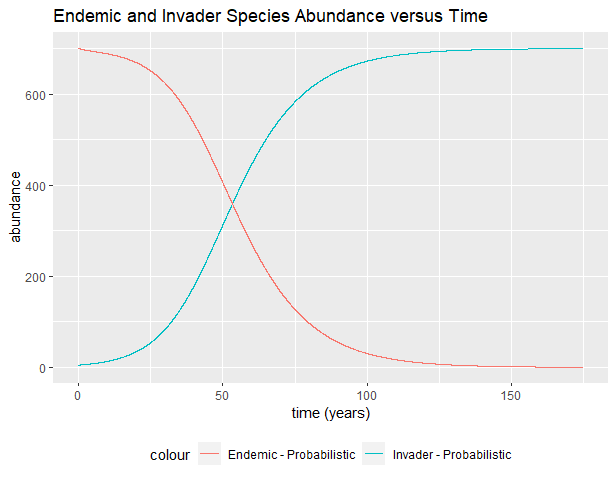
\includegraphics[scale=0.53]{determExample.png}
    \caption{Realization of Deterministic Model with TABLE 2 parameters}
    \label{fig:my_label}
\end{figure}

\end{document}